
\chapter{Graph neural networks}

The Graph Neural Network model~\cite{scarselli2009graph} (GNN) is a quite recent (2009) connectionist model, based on recursive neural networks and capable of classifying almost all types of graphs. The main difference between the GNN model and previous connectionist models is the possibility of processing directly nonpositional and cyclic graphs, containing both node labels and edge labels. Although some similar solutions were introduced in an earlier model, the \emph{RNN-LE}~\cite{bianchini2005recursive} in 2005, it was the GNN model that combined several techniques with a novel learning schema to provide a direct and flexible method for graph processing.

\section{Data}
The GNN model is built once for a training set of graphs. In fact, the whole training set can be merged into a large disconnected graph, which can be then fed to the model for learning. For a given dataset each node $n$ is described by a node label $\bm{l}_n$ of fixed size $|\bm{l}_n| \geq 1$. Each directed edge $u \Rightarrow n$ (from node $u$ to node $n$) is described by an edge label $\bm{l}_{(n, u)}$ of fixed size $|\bm{l}_{(n, u)}| \geq 0$. To deal with both directed and undirected edges, the authors propose to include a value $d_l$ in each edge label, denoting the direction of an edge. However, for a maximally general model, in this implementation all the edges were considered as directed. Undirected edges should be thus encoded prior to processing as pairs of directed edges with same labels.

A GNN model can deal with both \emph{graph-focused} and \emph{node-focused} tasks. In graph-focused tasks, for each graph an output $\bm{o}_n$ of fixed size $|\bm{o}_n| \geq 1$ is sought, which can denote e.g. the class of the graph. In the domain of chemistry, where each graph describes a chemical compound, this could describe e.g. the reactivity of a compound. In node-focused tasks, such output $\bm{o}_n$ is sought for every node in every graph. An example of such a task can be the face localisation problem, where for each region of an image the classifier should determine, if it belongs to the face or not. In the rest of this thesis, the \emph{node-focused} task is described, unless stated otherwise.

\section{Computation units}
The GNN model consists of two computation units, $f_{\bm{w}}$ and $g_{\bm{w}}$, where the $_{\bm{w}}$ subscript denotes the fact that both functions are parametrized by a vector of parameters $\bm{w}$, which is separate for the $f$ and for the $g$ function. The $f_{\bm{w}}$ unit is used for building representation (the \emph{state}) $\bm{x}_n$ of a single node $n$. The $g_{\bm{w}}$ unit is used for generating output $\bm{o}_n$ for a node $n$, basing on its representation $\bm{x}_n$. For a graph-focused task, the representation of the root node is fed to the $g_{\bm{w}}$ function to generate an output for the whole graph. It is important to remind, that for a given classifier there is only one $f_{\bm{w}}$ unit and one $g_{\bm{w}}$ unit (like in the recursive neural network model). All instances of the $f_{\bm{w}}$ unit share their weights and all instances of the $g_{\bm{w}}$ unit share their weights.

Let's denote by $ne[n]$ the neighbors of node $n$, that is such nodes $u$ that are connected to node $n$ by a directed edge $u \Rightarrow n$. Let's further denote by $co[n]$ the set of directed edges pointing from $ne[n]$ towards node $n$ (edges $u \Rightarrow n$). The general forms of $f_{\bm{w}}$ and $g_{\bm{w}}$ functions are defined by equations Eq.~\ref{eq:gnn_f} and Eq.~\ref{eq:gnn_g}, where $\bm{l}_n$ denotes the $n$th node label, $\bm{l}_{co[n]}$ denotes vector of edge labels from $co[n]$ stacked one after another, $\bm{x}_{ne[n]}$ denotes \emph{states} of nodes from $ne[n]$, and $\bm{l}_{ne[n]}$ denotes their labels.

\begin{equation}
\bm{x}_n = f_{\bm{w}}(\bm{l}_n, \; \bm{l}_{co[n]}, \; \bm{x}_{ne[n]}, \; \bm{l}_{ne[n]})
\label{eq:gnn_f}
\end{equation}

\begin{equation}
\bm{o}_n = g_{\bm{w}}(\bm{x}_n, \; \bm{l}_n)
\label{eq:gnn_g}
\end{equation}

\noindent For this implementation, a minimal version of these definitions was chosen, as shown in Eq.~\ref{eq:gnn_fmin} and Eq.~\ref{eq:gnn_gmin}.

\begin{equation}
\bm{x}_n = f_{\bm{w}}(\bm{l}_n, \; \bm{l}_{co[n]}, \; \bm{x}_{ne[n]})
\label{eq:gnn_fmin}
\end{equation}

\begin{equation}
\bm{o}_n = g_{\bm{w}}(\bm{x}_n)
\label{eq:gnn_gmin}
\end{equation}

These forms were chosen to prove that the model is capable of building a sufficient representation of each node. That is, the model should be able to encode the necessary information from a node label $\bm{l}_n$ into the state $\bm{x}_n$. This approach proved to be successful as the first experiment, consisting of a classification task basing on node labels only, yielded perfect results.

From two forms of the $f_{\bm{w}}$ function mentioned in the original article~\cite{scarselli2009graph}, the \emph{nonpositional form} was chosen. The reason was to provide the model with the most general function available, which could deal with both positional and nonpositional graphs. The nonpositional form was also the one yielding better results in the experiments conducted by the authors~\cite{scarselli2009graph}. The equations Eq.~\ref{eq:gnn_ffinal} and Eq.~\ref{eq:gnn_gfinal} show the final equations describing the $f_{\bm{w}}$ and $g_{\bm{w}}$ functions. All instances of the $h_{\bm{w}}$ unit share their weights.

\begin{equation}
\bm{x}_n = \sum_{u \in ne[n]}h_{\bm{w}}(\bm{l}_n, \; \bm{l}_{(n,u)}, \; \bm{x}_{u})
\label{eq:gnn_ffinal}
\end{equation}

\begin{equation}
\bm{o}_n = g_{\bm{w}}(\bm{x}_n)
\label{eq:gnn_gfinal}
\end{equation}

The units $h_{\bm{w}}$ and $g_{\bm{w}}$ were implemented as fully-connected three layer feed-forward neural networks (input lines performing no computation, a single hidden layer and an output layer). For both units the hidden layer consisted of $tanh$ neurons. For the $h_{\bm{w}}$ unit the output layer consisted also of $tanh$ neurons. That's because the output of this unit contributes to the state value and therefore should consist of bounded values only. For the $g_{\bm{w}}$ unit the output layer could consist either of $tanh$ or linear neurons, depending on the values of $\bm{o}_n$ that should be learned.

At this point it's worth noting that the final value of $\bm{x}_n$ is calculated as a simple sum of $h_{\bm{w}}$ outputs. This corresponds to a situation where all the $h_{\bm{w}}$ output values are passed to a neural network in which the set of weights corresponding to a single $h_{\bm{w}}$ input are shared amongst all the $h_{\bm{w}}$ inputs. If we consider that a three layer FNN used as $h_{\bm{w}}$ unit is already an universal approximator, the use of such an additional neural network which just sums all $h_{\bm{w}}$ values using the same shared set of weights is unnecessary. A simple sum should be sufficient and experimental results showed that this assumption stands.

The $f_{\bm{w}}$ and $g_{\bm{w}}$ units are presented in Fig.~\ref{fig:gnn_f} and Fig.~\ref{fig:gnn_g}, where the comma-separated list of inputs stands for a vector obtained by stacking all the listed values one after another.

\begin{figure}
\begin{center}
	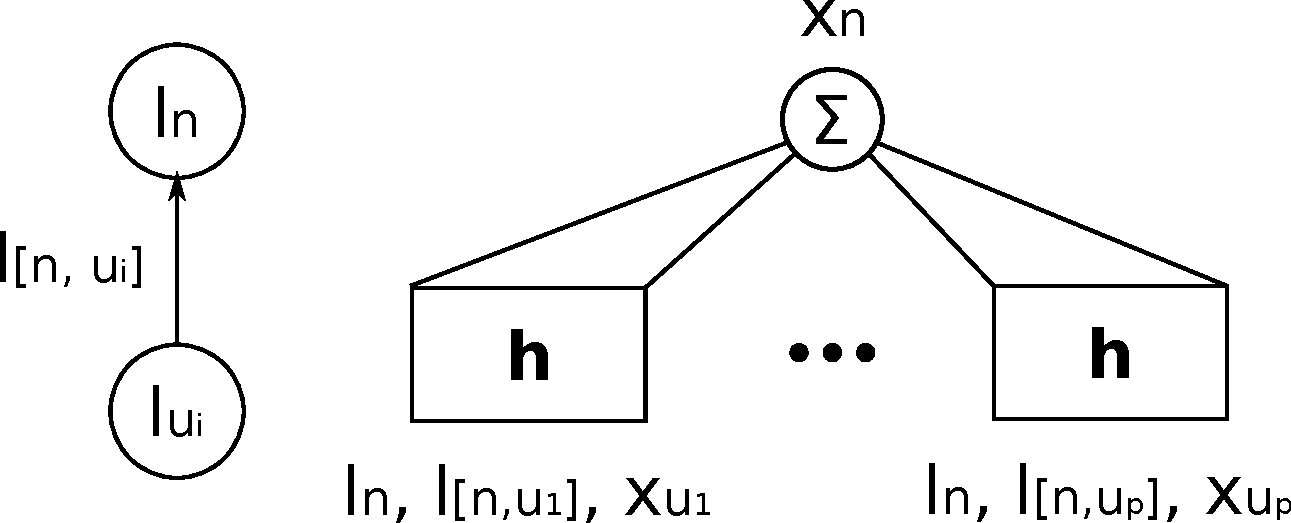
\includegraphics[scale=0.6]{img/f_ext}
	\caption{The $f_{\bm{w}}$ unit for a single node with one of the corresponding edges}
	\label{fig:gnn_f}
\end{center}
\end{figure}

\begin{figure}
\begin{center}
	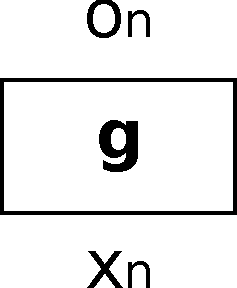
\includegraphics[scale=0.6]{img/g}
	\caption{The $g_{\bm{w}}$ unit for a single node}
	\label{fig:gnn_g}
\end{center}
\end{figure}

The weights of both the $h_{\bm{w}}$ and $g_{\bm{w}}$ units were initialised according to standard neural network practice, to avoid saturation of any $tanh$ activation function: $net_j = \sum_i w_{ij} y_i \in (-1, 1)$, where $net_j$ is the weighted input to $j$th neuron, $y_i$ is the $i$th input value and $w_{ij}$ is the weight corresponding to the $i$th input. The initial input weights of the $g_{\bm{w}}$ unit were divided by an additional factor, i.e. the maximum node indegree of the processed graphs, to take into consideration the fact, that the input of $g_{\bm{w}}$ unit consists of a sum of $h_{\bm{w}}$ outputs. All the input data (node and edge labels) was normalised appropriately before feeding to the model.


\section{The encoding network}
Graph processing by a GNN model consists of two steps: building representation $\bm{x}_n$ for each node and producing an output $\bm{o}_n$. As the representation of a single node depends on other nodes representations, an encoding network for every graph is be built, reflecting the structure of the graph. The encoding network consists of instances of the $f_{\bm{w}}$ unit connected according to the graph connectivity with a $g_{\bm{w}}$ unit attached to every $f_{\bm{w}}$ unit. A sample graph and its encoding network are presented in Fig.~\ref{fig:gnn_encoding}.
It can be seen that, as a cyclic dependence exists in the sample graph, the calculation of the node \emph{states} should be iterative, until at some point convergence is reached.

\begin{figure}[h!]
\begin{center}
	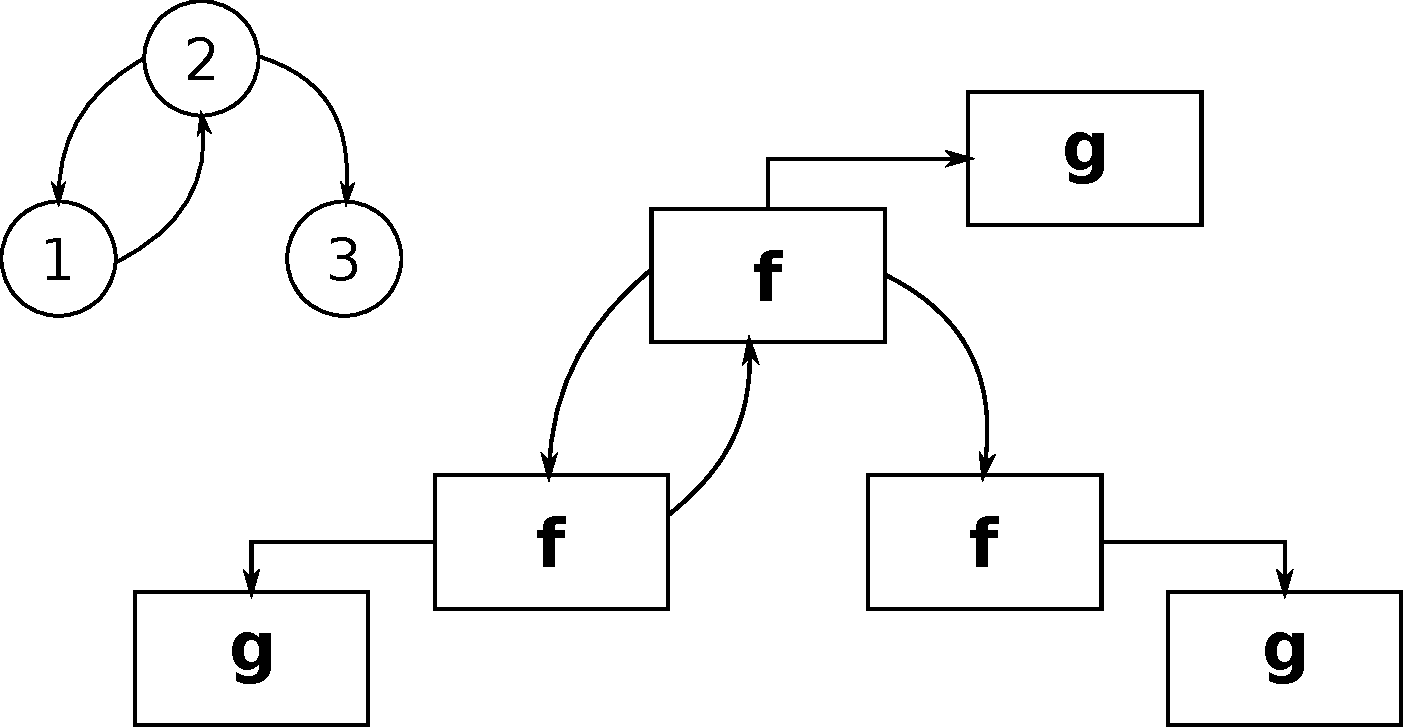
\includegraphics[scale=0.4]{img/encodinginc}
	\caption{A sample graph and the corresponding encoding network}
	\label{fig:gnn_encoding}
\end{center}
\end{figure}


\section{The training algorithm}
To solve the problem of cyclic dependencies, the GNN models adapts a novel learning algorithm for the encoding network. Let's denote by $x$ the \emph{global state} of the graph, that is the set of $\bm{x}_n$ for every node $n$ in the graph. Let's denote by $\bm{l}$ and $\bm{o}$ the sets of all labels and all outputs, respectively. Let's further denote by $F_{\bm{w}}$ and $G_{\bm{w}}$ (\emph{global transition function} and \emph{global output function}) the stacked versions of $f_{\bm{w}}$ and $g_{\bm{w}}$ functions, respectively. Now, equations~\ref{eq:gnn_fmin} and~\ref{eq:gnn_gmin} can be rewritten as Eq.~\ref{eq:gnn_fglobal} and Eq.~\ref{eq:gnn_gglobal}.

\begin{equation}
\bm{x} = F_{\bm{w}}(\bm{l}, \; \bm{x})
\label{eq:gnn_fglobal}
\end{equation}

\begin{equation}
\bm{o} = G_{\bm{w}}(\bm{x})
\label{eq:gnn_gglobal}
\end{equation}

\noindent The GNN training algorithm can be described as follows:
\begin{enumerate}
	\item initialize $h_{\bm{w}}$ and $g_{\bm{w}}$ weights
	\item until stop criterion is satisfied:
	\begin{enumerate}
		\item initialize $X$ randomly
		\item FORWARD: calculate $X = F(X)$ until convergence
		\item BACKWARD: calculate $G(X)$ and backpropagate the error
		\item update $h_{\bm{w}}$ and $g_{\bm{w}}$ weights
	\end{enumerate}
\end{enumerate}



